\documentclass[conference]{IEEEtran}
\usepackage[utf8]{inputenc}
\usepackage[T1]{fontenc}
\usepackage{amsmath,amssymb}
\usepackage{graphicx}
\usepackage{booktabs}
\usepackage{multirow}
\usepackage{hyperref}

\title{Symbolic Logic, Adversarial Search, and Constraint Satisfaction Solvers for Classical AI Problems}

\author{
\IEEEauthorblockN{Team Leader Full Name (Student ID), Quy Full Name (Student ID),\\
Huynh Thien Duc (Student ID), Le Tien Dat (Student ID), and Thanh-An Nguyen}
\IEEEauthorblockA{Faculty of Information Technology, Ton Duc Thang University, Ho Chi Minh City, Vietnam\\
Emails: \{leader, quy, duc, dat\}@student.tdtu.edu.vn, nguyenthanhan@tdtu.edu.vn}
}

\begin{document}
\maketitle

\begin{abstract}
This paper presents an object-oriented design and experimental evaluation of three foundational Artificial Intelligence paradigms developed for Course 503043. In Task 1, we formulate the $N$-Queen problem in Propositional Logic, derive a closed-form Conjunctive Normal Form (CNF) encoding solved via \texttt{Glucose3}, and propose a \emph{Max-Conflict with Short-Term Tabu and Aspiration} heuristic that cuts average repair steps from $107.2$ to $63.3$ at $N=64$. In Task 2, we formalize a turn-based Tank Battle game with immutable states and persistent 3-cell-per-cycle projectile physics as a Zero-Sum Game, benchmark four adversarial search configurations (Minimax, Alpha-Beta, Heuristic Minimax, and Heuristic Alpha-Beta with Move Ordering and Transposition Tables), and build a responsive PyGame arena supporting dynamic external bot plugins. In Task 3, we model Kakuro puzzles as Constraint Satisfaction Problems (CSPs) combining Sum-Partition preprocessing, Extended AC-3 propagation, and MRV/Degree/LCV heuristics, solving all four benchmark boards ($5\times 5$ to $9\times 9$, up to $48$ variables) with zero backtracks alongside a threaded PyGame visualizer and interactive board editor.
\end{abstract}

\begin{IEEEkeywords}
Propositional Logic, PySAT Glucose3, Min-Conflicts, Adversarial Search, Alpha-Beta Pruning, Kakuro CSP.
\end{IEEEkeywords}

\section{Task 1: N-Queen via Propositional Logic and Min-Conflicts}

\subsection{Propositional Formulation and CNF Conversion}
Given an $N \times N$ chessboard, we assign a Boolean variable $P_{r,c} \in \{\text{True}, \text{False}\}$ to each square $(r, c) \in \{0, \dots, N-1\}^2$, mapped bijectively to DIMACS integer $\text{id}(r, c) = rN + c + 1 \in \{1, \dots, N^2\}$ \cite{russell2020aima}. Valid placements are governed by two axiom families:
\begin{enumerate}
    \item \emph{Existence (At-Least-One)}: Every row $r$ and column $c$ contains at least one queen: $\bigvee_{c=0}^{N-1} P_{r,c}$ and $\bigvee_{r=0}^{N-1} P_{r,c}$.
    \item \emph{Non-Attacking (Pairwise Implication)}: For every distinct pair $(r_1, c_1) \prec (r_2, c_2)$ sharing a row ($r_1 = r_2$), column ($c_1 = c_2$), main diagonal ($r_1 - c_1 = r_2 - c_2$), or anti-diagonal ($r_1 + c_1 = r_2 + c_2$), placing a queen at $(r_1, c_1)$ forbids $(r_2, c_2)$: $P_{r_1,c_1} \Rightarrow \neg P_{r_2,c_2}$.
\end{enumerate}

Eliminating implication ($P_{r_1,c_1} \Rightarrow \neg P_{r_2,c_2} \equiv \neg P_{r_1,c_1} \vee \neg P_{r_2,c_2}$) yields binary CNF clauses directly without auxiliary Tseitin variables. Summing over rows, columns, and all $2N-1$ diagonals yields:
\begin{equation}
|C_{\text{CNF}}(N)| = 2N + N^2(N-1) + \frac{N(N-1)(2N-1)}{3}.
\end{equation}

\subsection{Glucose3 SAT Experiments and Proposed Tabu Min-Conflicts}
Using \texttt{Glucose3} \cite{audemard2009glucose,ignatiev2018pysat}, we evaluate $N \in [4, 60]$. As shown in Fig.~\ref{fig:task1_sat}, $|C_{\text{CNF}}|$ scales cubically as $\mathcal{O}(N^3)$, reaching $203{,}450$ clauses at $N=50$ ($93.9$~ms solve time) and $352{,}940$ clauses at $N=60$ ($166.2$~ms).

\begin{figure}[t]
    \centering
    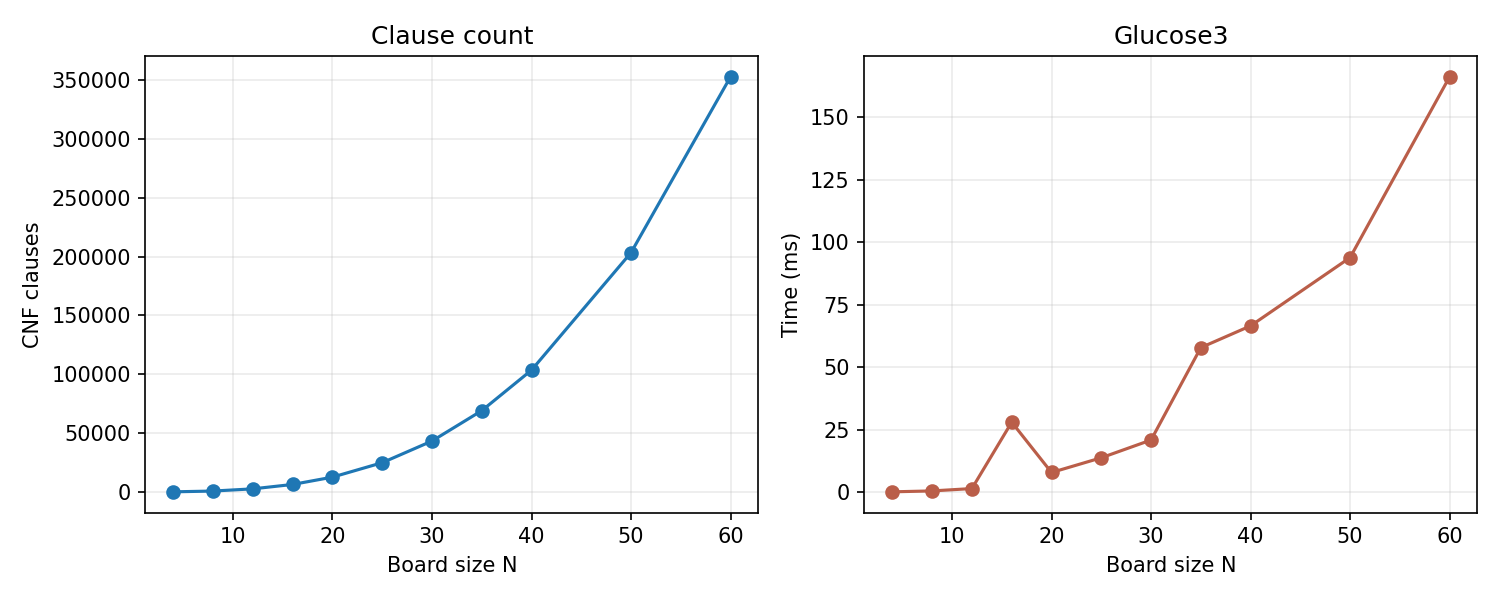
\includegraphics[width=0.95\columnwidth]{figures/task1_glucose3_scaling.png}
    \caption{CNF clause growth and \texttt{Glucose3} runtime across $N \in [4, 60]$.}
    \label{fig:task1_sat}
\end{figure}

For Local Search, complete states $\text{queens}[c] = r$ place one queen per column with $\mathcal{O}(1)$ incremental row and diagonal counters \cite{minton1992minconflicts}. Our heuristic prioritizes maximally conflicted columns, prevents short-term cycling via a Tabu tenure $k = \max(2, \min(8, \lfloor 0.12N \rfloor))$, overrides Tabu when an aspiration move eliminates all board conflicts, and resets after $16$ stagnant steps. Across $30$ shared random initial boards per size ($2{,}500$-step cap, Fig.~\ref{fig:task1_mc}), both methods achieve $100\%$ success for $N \ge 16$, while our heuristic reduces mean steps from $96.0 \to 30.7$ ($N=16$), $107.2 \to 63.3$ ($N=64$), and $179.5 \to 125.1$ ($N=150$). An interactive Tkinter chessboard interface (\texttt{gui.py}) is also provided.

\begin{figure}[t]
    \centering
    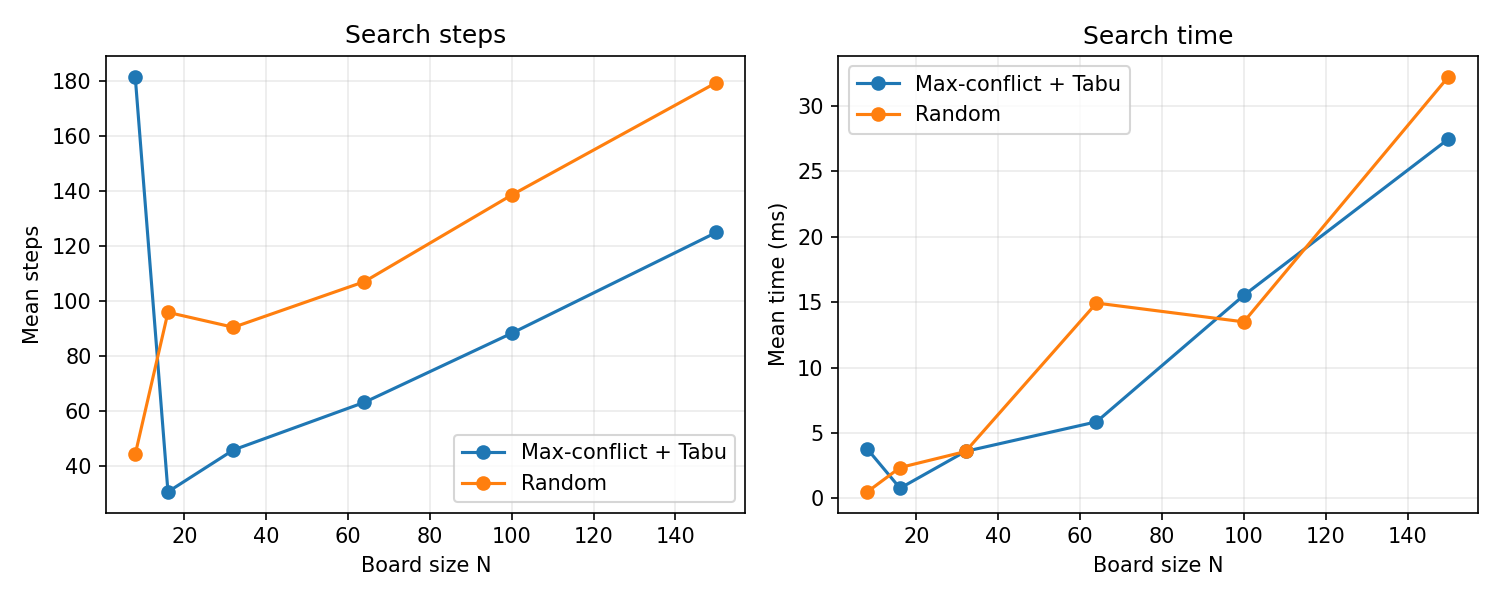
\includegraphics[width=0.95\columnwidth]{figures/task1_min_conflicts_comparison.png}
    \caption{Standard Min-Conflicts vs. Proposed Max-Conflict + Tabu heuristic.}
    \label{fig:task1_mc}
\end{figure}

\section{Task 2: Tank Battle via Zero-Sum Adversarial Search}

\subsection{Zero-Sum Game Formulation and Heuristic Optimization}
Tank Battle is formalized as a deterministic two-player Zero-Sum Game $\mathcal{G} = \langle S_0, \text{PLAYER}, \text{ACTIONS}, \text{RESULT}, \text{TERMINAL}, \text{UTILITY} \rangle$ \cite{russell2020aima,knuth1975alphabeta} over immutable state snapshots. Entities match specification health values: Tank ($\text{HP}=6$), Base ($\text{HP}=9$), and Brick Wall ($\text{HP}=3$), with $1$ damage per hit and action set $\{\texttt{MOVE\_UP}, \texttt{MOVE\_DOWN}, \texttt{MOVE\_LEFT}, \texttt{MOVE\_RIGHT}, \texttt{FIRE}, \texttt{STAY}\}$. Directional actions update orientation and advance $1$ cell if unobstructed; active bullets persist across turns and advance up to $3$ cells per cycle with sequential cell-by-cell collision checks. Terminal states yield $+1000$ ($\text{MAX}$ win), $-1000$ ($\text{MIN}$ win), or $0$ (draw).

Depth-limited search evaluates non-terminal leaves at cutoff $d$ via:
\begin{align}
\text{EVAL}(s) &= 125\Delta\text{HP}_{\text{tank}} + 155\Delta\text{HP}_{\text{base}} + 4.5\Delta d_{\text{base}} \nonumber\\
&\quad + 24\Delta\text{LoF}(s) + \Delta\text{Breach}(s) - 65\Delta\text{Threat}(s),
\end{align}
combined with tactical \emph{Move Ordering} and a canonical \emph{Transposition Table}.

\subsection{Two-Tier Benchmark and PyGame Plugin Arena}
To compare all four configurations fairly, Tier-1 uses low-HP $7\times 7$ tactical endgames where exact search reaches terminal states, while Tier-2 evaluates full-HP $9\times 9$ and $11\times 11$ arenas. On \emph{Endgame Center Duel}, Pure Minimax explores $30{,}278$ states ($974.1$~ms), Pure Alpha-Beta explores $2{,}213$ states ($69.4$~ms) for the identical optimal move, Heuristic Minimax ($d=4$) explores $1{,}004$ states ($56.5$~ms), and Heuristic Alpha-Beta explores $34$ states ($2.2$~ms)---an $890\times$ state reduction (Fig.~\ref{fig:task2_bench}). At depth $4$ on Tier-2 arenas (Fig.~\ref{fig:task2_tier2}), Heuristic Alpha-Beta searches $94$ states on Classic $9\times 9$ ($5.9$~ms, $5$ TT hits) and $212$ states on Fortress $11\times 11$ ($22.3$~ms, $17$ TT hits), versus $895$ and $1{,}478$ states for Heuristic Minimax. Our PyGame GUI (Fig.~\ref{fig:task2_ui}) integrates Kenney's CC0 sprites~\cite{kenneyTopDownTanksRedux} and dynamically loads external bots via \texttt{BaseTankAgent} subclasses or dictionary adapters.

\begin{figure}[t]
    \centering
    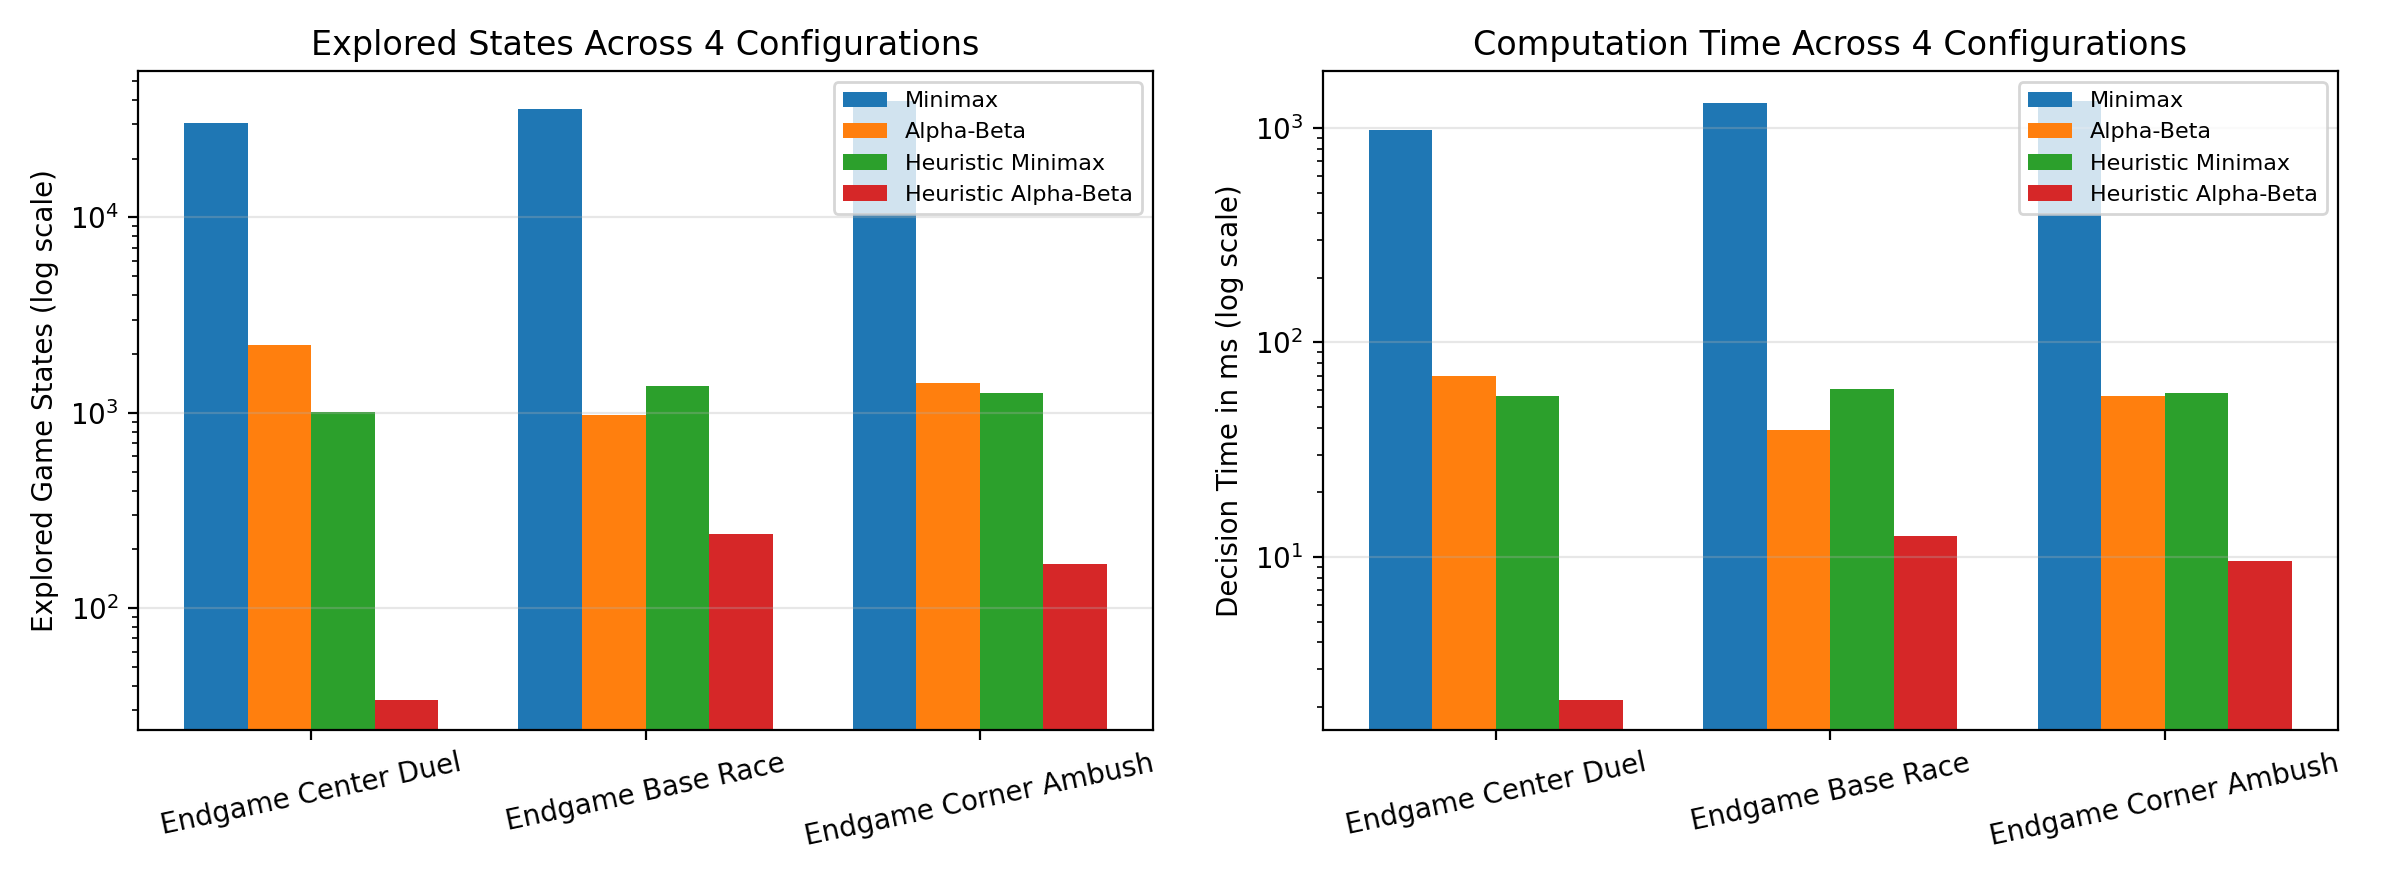
\includegraphics[width=0.95\columnwidth]{figures/task2_four_algo_comparison.png}
    \caption{Explored states and decision time across all 4 search configurations.}
    \label{fig:task2_bench}
\end{figure}

\begin{figure*}[t]
    \centering
    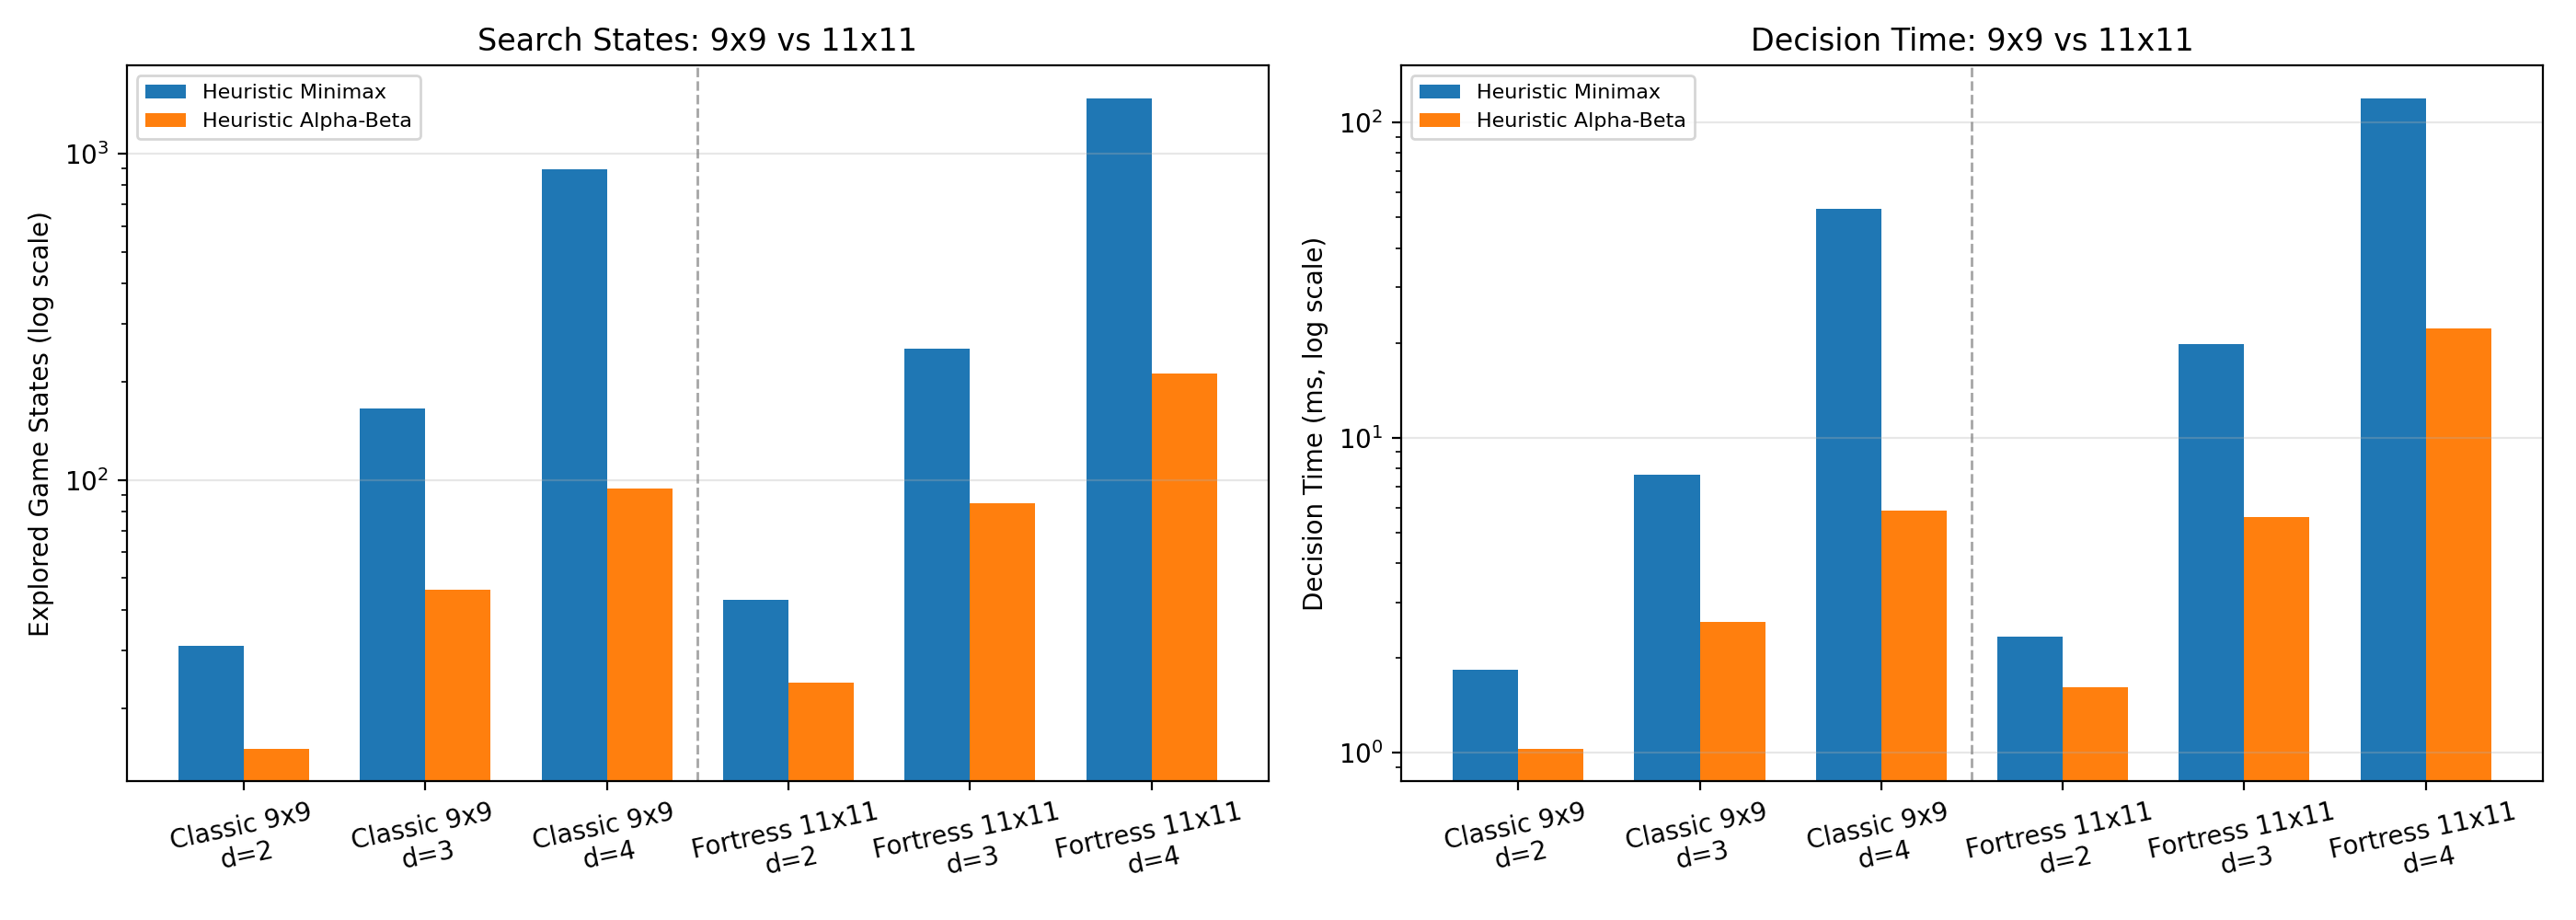
\includegraphics[width=0.86\textwidth]{figures/task2_tier2_9x9_vs_11x11.png}
    \caption{Tier-2 search states and decision time on Classic $9\times 9$ and Fortress $11\times 11$ arenas across depths $d \in \{2, 3, 4\}$.}
    \label{fig:task2_tier2}
\end{figure*}

\begin{figure}[t]
    \centering
    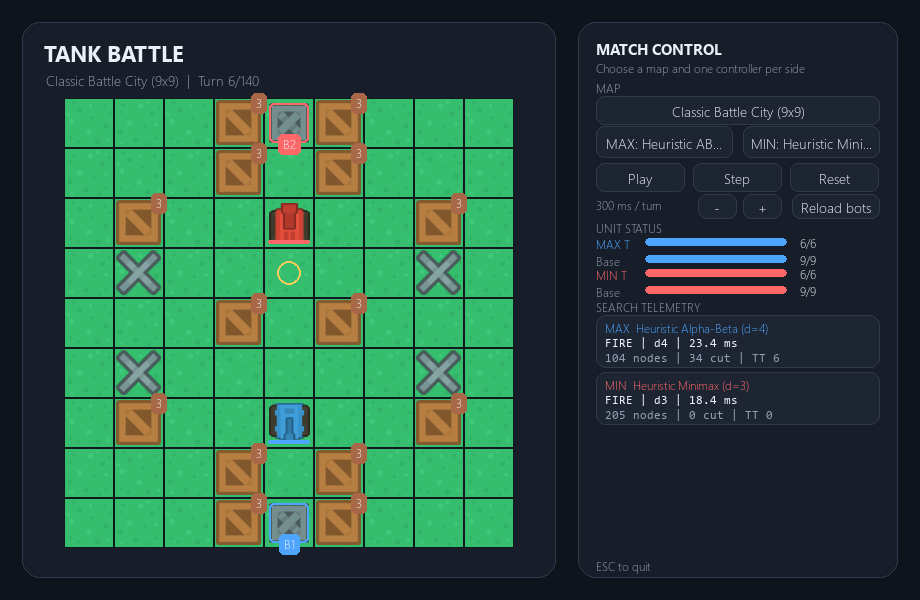
\includegraphics[width=0.92\columnwidth]{figures/task2_arena_ui.png}
    \caption{Responsive two-column PyGame arena with live search telemetry.}
    \label{fig:task2_ui}
\end{figure}

\section{Task 3: Kakuro Puzzle as a Constraint Satisfaction Problem}

\subsection{CSP Formulation, Propagation, and Heuristics}
Kakuro is modeled as $\langle X, D, C \rangle$ \cite{simonis2008kakuro}, where $X$ comprises all white squares ($|X|=12$ on the $5\times 5$ example; $|X|=48$ on the $9\times 9$ complex test case), domains $D_i \subseteq \{1,\dots,9\}$ are pre-filtered via \emph{Sum-Partition} intersections, and each contiguous run $r$ of length $k$ and clue $S$ enforces both $\text{AllDiff}(X_r)$ and $\sum_{x \in X_r} x = S$. Our advanced solver combines Forward Checking and \emph{Extended AC-3} (generalized arc support with tight residual min/max bounds) with \textbf{MRV}, \textbf{Degree} tie-breaking, and 1-hop \textbf{LCV} ordering.

\subsection{Statistical Evaluation, Visualizer UI, and Board Editor}
Across $30$ trials per configuration on four boards ($5\times 5$, $6\times 6$, $8\times 8$, $9\times 9$), all solutions pass $100\%$ constraint verification (Table~\ref{tab:kakuro}, Fig.~\ref{fig:task3_bench}). On the $9\times 9$ test case, Baseline Backtracking explores $9{,}141$ nodes ($988$ backtracks, $69.3$~ms), \texttt{BT + FC + MRV} explores $100$ nodes ($52$ backtracks, $6.1$~ms), and \texttt{BT + Ext.\ AC-3 + MRV/Degree/LCV} solves all $48$ variables in $48$ nodes ($0$ backtracks, $43.8$~ms---a $99.48\%$ node reduction). Our PyGame UI executes search on a cancellable background thread, visualizes $3\times 3$ candidate grids, pruning, and backtracks step-by-step, and includes an interactive \texttt{BoardEditor} supporting given digits, bulk editing, clue randomization, and JSON persistence.

\begin{table}[t]
\centering
\caption{Kakuro CSP Mean Performance (30 Trials per Mode)}
\label{tab:kakuro}
\resizebox{\columnwidth}{!}{%
\begin{tabular}{lcccc}
\toprule
\textbf{Board ($|X|$)} & \textbf{Solver Mode} & \textbf{Nodes} & \textbf{Backtracks} & \textbf{Time (ms)} \\
\midrule
\multirow{3}{*}{$5\times 5$ Spec (12)} & Baseline BT & 9,933 & 1,097 & $61.8 \pm 17.9$ \\
 & BT + FC + MRV & 13 & 1 & $0.7 \pm 0.2$ \\
 & BT + Ext. AC-3 + Heuristics & \textbf{12} & \textbf{0} & $3.6 \pm 1.7$ \\
\midrule
\multirow{3}{*}{$9\times 9$ Complex (48)} & Baseline BT & 9,141 & 988 & $69.3 \pm 10.7$ \\
 & BT + FC + MRV & 100 & 52 & $6.1 \pm 0.8$ \\
 & BT + Ext. AC-3 + Heuristics & \textbf{48} & \textbf{0} & $43.8 \pm 3.6$ \\
\bottomrule
\end{tabular}%
}
\end{table}

\begin{figure}[t]
    \centering
    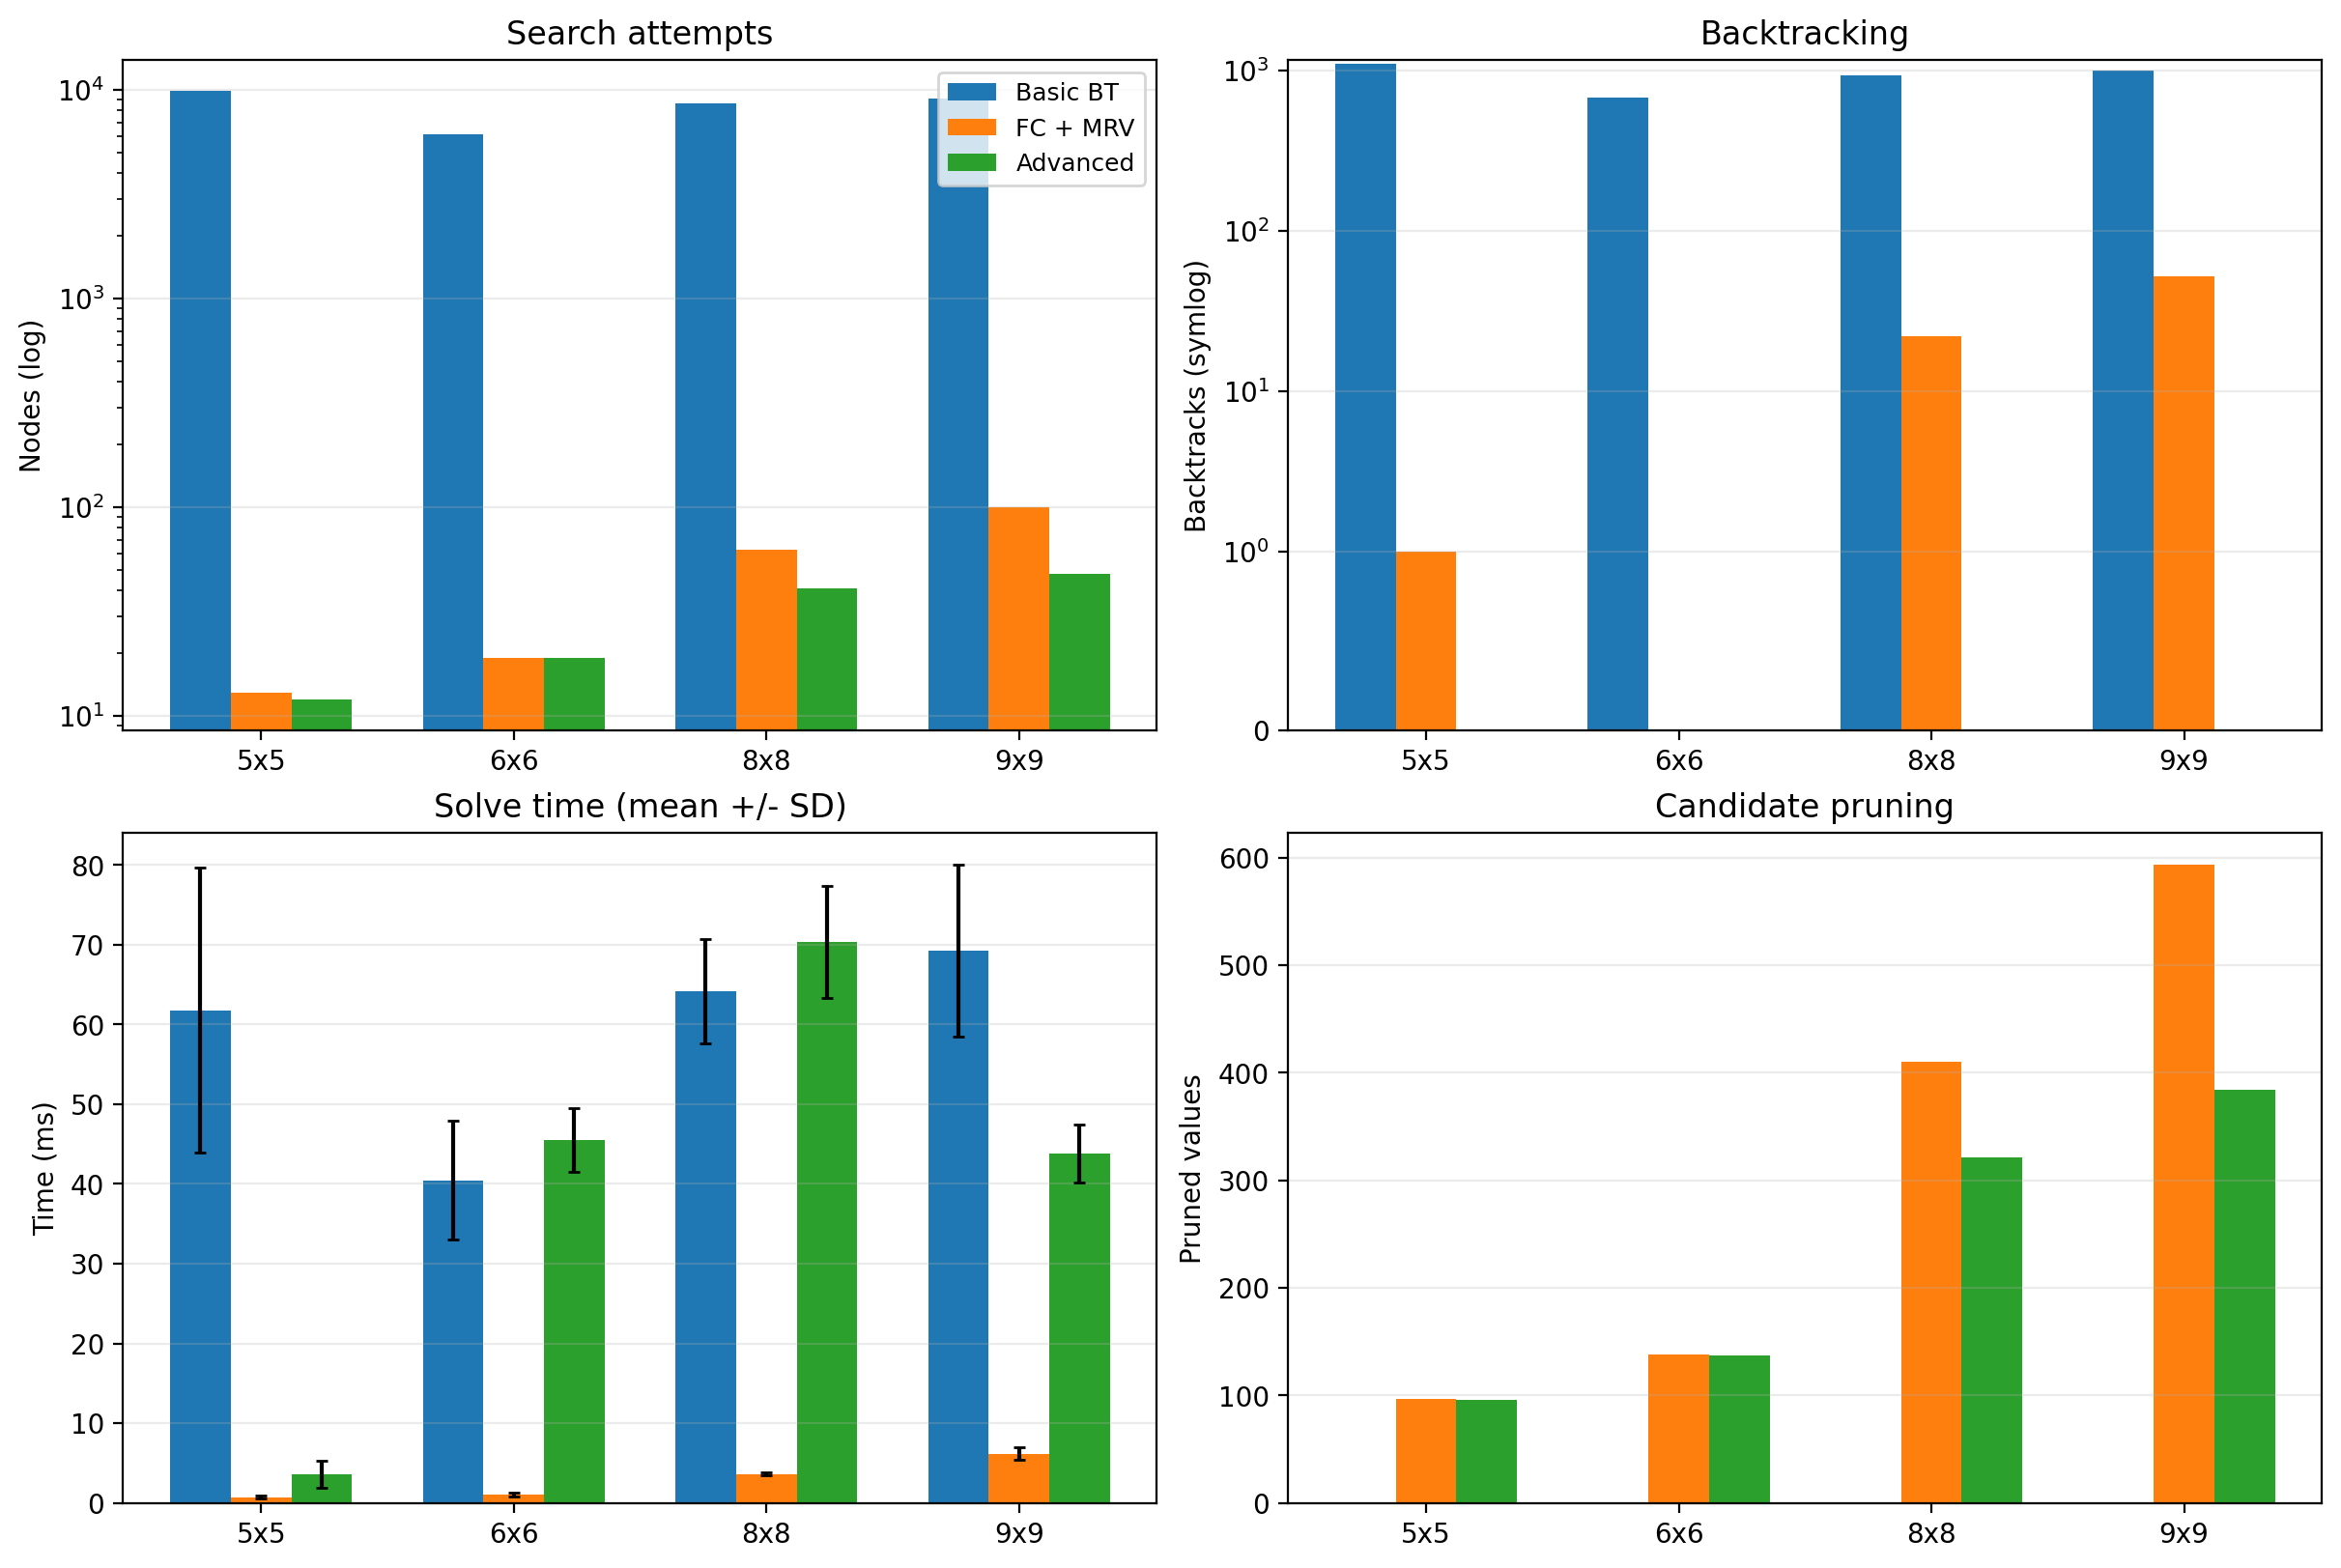
\includegraphics[width=0.95\columnwidth]{figures/task3_csp_benchmark.png}
    \caption{Mean nodes, backtracks, solve time, and pruned candidates across four Kakuro boards.}
    \label{fig:task3_bench}
\end{figure}

\section{Contributions and Self-Evaluation}

\subsection{Individual Contributions}
\begin{itemize}
    \item \textbf{Team Leader (100\% assigned)}: Overall OOP architecture, Git branch integration, cross-platform compatibility verification (macOS 13.7.8), IEEE report synthesis, and demo coordination.
    \item \textbf{Quy (100\% assigned)}: Task 1 CNF encoder, \texttt{Glucose3} experiments, Tabu Min-Conflicts heuristic, Tkinter chessboard GUI (\texttt{gui.py}), and Task 1 notebook analysis.
    \item \textbf{Huynh Thien Duc (100\% assigned)}: Task 2 immutable Zero-Sum engine, four search agents, tactical evaluator, PyGame Arena \& external bot plugin loader, and two-tier benchmarks.
    \item \textbf{Le Tien Dat (100\% assigned)}: Task 3 Kakuro CSP model, Sum-Partition \& Extended AC-3 propagators, MRV/Degree/LCV solver, PyGame visualizer \& \texttt{BoardEditor}, and 30-trial statistical benchmarks.
\end{itemize}

\subsection{Self-Evaluation}
All theoretical formulations, OOP implementations, interactive GUIs, and reproducible notebooks are $100\%$ complete: Task 1 ($3.0/3.0$), Task 2 ($3.0/3.0$), Task 3 ($3.0/3.0$), and Task 4 ($1.0/1.0$), for an estimated total score of $\mathbf{10.0 / 10.0}$.

\section{Conclusion}
We designed, implemented, and experimentally validated OOP solvers across Propositional Logic SAT, Local Search, Zero-Sum Adversarial Search, and Constraint Satisfaction Problems. Combining structural domain propagation with informed variable and value ordering reduced search complexity by orders of magnitude while maintaining responsive interactive interfaces.

\bibliographystyle{IEEEtran}
\bibliography{references}

\end{document}
